\documentclass{article}

\usepackage{fancyhdr}
\usepackage{extramarks}
\usepackage{amsmath}
\usepackage{amsthm}
\usepackage{amsfonts}
\usepackage{tikz}
\usepackage{graphicx} %插入图片的宏包
\usepackage{float} %设置图片浮动位置的宏包
\usepackage{pythonhighlight}
% \usepackage{subfigure} %插入多图时用子图显示的宏包
% \usepackage[plain]{algorithm}
% \usepackage{algpseudocode}

% \usetikzlibrary{automata,positioning}

%
% Basic Document Settings
%

\topmargin=-0.45in
\evensidemargin=0in
\oddsidemargin=0in
\textwidth=6.5in
\textheight=9.0in
\headsep=0.25in

\linespread{1.1}

\pagestyle{fancy}
\lhead{\hmwkAuthorName}
\chead{\hmwkClass\ : \hmwkTitle}
\rhead{\firstxmark}
\lfoot{\lastxmark}
\cfoot{\thepage}

\renewcommand\headrulewidth{0.4pt}
\renewcommand\footrulewidth{0.4pt}

\setlength\parindent{0pt}


%代码格式设置



%
% Create Problem Sections
%

\newcommand{\enterProblemHeader}[1]{
    \nobreak\extramarks{}{Problem \arabic{#1} continued on next page\ldots}\nobreak{}
    \nobreak\extramarks{Problem \arabic{#1} (continued)}{Problem \arabic{#1} continued on next page\ldots}\nobreak{}
}

\newcommand{\exitProblemHeader}[1]{
    \nobreak\extramarks{Problem \arabic{#1} (continued)}{Problem \arabic{#1} continued on next page\ldots}\nobreak{}
    \stepcounter{#1}
    \nobreak\extramarks{Problem \arabic{#1}}{}\nobreak{}
}

\setcounter{secnumdepth}{0}
\newcounter{partCounter}
\newcounter{homeworkProblemCounter}
\setcounter{homeworkProblemCounter}{1}
\nobreak\extramarks{Problem \arabic{homeworkProblemCounter}}{}\nobreak{}

%
% Homework Problem Environment
%
% This environment takes an optional argument. When given, it will adjust the
% problem counter. This is useful for when the problems given for your
% assignment aren't sequential. See the last 3 problems of this template for an
% example.
%
\newenvironment{homeworkProblem}[1][-1]{
    \ifnum#1>0
        \setcounter{homeworkProblemCounter}{#1}
    \fi
    \section{Problem \arabic{homeworkProblemCounter}}
    \setcounter{partCounter}{1}
    \enterProblemHeader{homeworkProblemCounter}
}{
    \exitProblemHeader{homeworkProblemCounter}
}

%
% Homework Details
%   - Title
%   - Due date
%   - Class
%   - Section/Time
%   - Instructor
%   - Author
%

\newcommand{\hmwkTitle}{Quiz\ \#7}
\newcommand{\hmwkDueDate}{Dec 31, 2018}
\newcommand{\hmwkClass}{Complex Networks}
\newcommand{\hmwkClassTime}{Section A}
% \newcommand{\hmwkClassInstructor}{Professor Isaac Newton}
\newcommand{\hmwkAuthorName}{\textbf{RUOPENG XU} }
\newcommand{\hmwkAuthorNum}{\textbf{18M38179} }

%
% Title Page
%

\title{
    \vspace{2in}
    \textmd{\textbf{\hmwkClass:\ \hmwkTitle}}\\
    \normalsize\vspace{0.1in}\small{Due\ on\ \hmwkDueDate\ }\\
    % \vspace{0.1in}\large{\textit{\hmwkClassInstructor\ \hmwkClassTime}}
    \vspace{3in}
}

\author{\hmwkAuthorName\\ \hmwkAuthorNum}
\date{}

\renewcommand{\part}[1]{\textbf{\large Part \Alph{partCounter}}\stepcounter{partCounter}\\}

%
% Various Helper Commands
%

% Useful for algorithms
\newcommand{\alg}[1]{\textsc{\bfseries \footnotesize #1}}

% For derivatives
\newcommand{\deriv}[1]{\frac{\mathrm{d}}{\mathrm{d}x} (#1)}

% For partial derivatives
\newcommand{\pderiv}[2]{\frac{\partial}{\partial #1} (#2)}

% Integral dx
\newcommand{\dx}{\mathrm{d}x}

% Alias for the Solution section header
\newcommand{\solution}{\textbf{\large Solution}}

% Probability commands: Expectation, Variance, Covariance, Bias
\newcommand{\E}{\mathrm{E}}
\newcommand{\Var}{\mathrm{Var}}
\newcommand{\Cov}{\mathrm{Cov}}
\newcommand{\Bias}{\mathrm{Bias}}

\begin{document}

\maketitle

\pagebreak

\begin{homeworkProblem}
    % questions
Make a program of computing degree assortativity of Karate
club network.

% 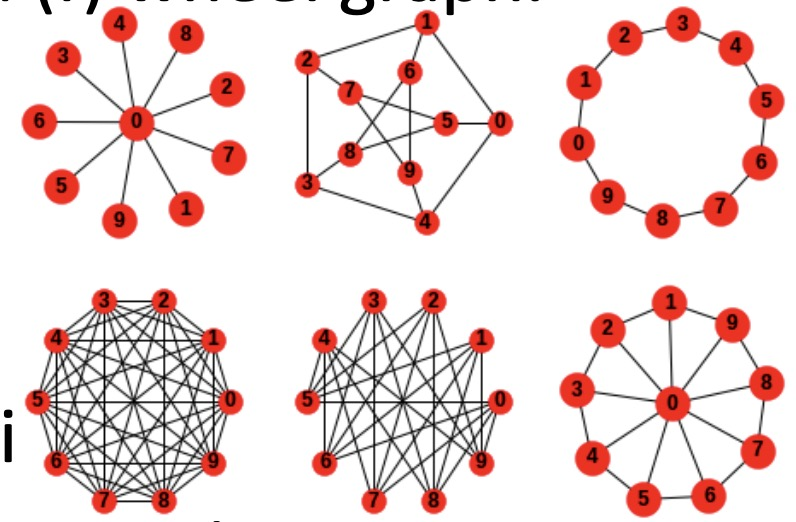
\includegraphics[scale=0.3]{quiz6_1.jpg}

\subsection*{Answer 1}

\begin{python}
import networkx as nx

G = nx.karate_club_graph()
result = nx.degree_assortativity_coefficient(G)
print("the degree assortativity of karate club is", result)
\end{python}

The result is:
\begin{python}
the degree assortativity of karate club is -0.47561309768461457
\end{python}







\end{homeworkProblem}
\pagebreak


\begin{homeworkProblem}
What are the input(s) and output(s) of modularity? What
does the output(s) mean?
\subsection*{Answer 2}

As shown in the slide, the modularity is 
$\displaystyle Q = \frac{1}{2m} \sum_{ij}^{ }(A_{ij} - \frac{k_ik_j}{2m})\delta (c_i,c_j)$
\\
\\
The input is : 1.the Adjacency Matrix of the network; 2.the degree of each node; 3.whether node i and node j are in the same group; 4. the number of edges in the network.
\\
\\
The output is : the modularity, \textit{which measures the strength of division of a network into groups. Networks with high modularity have dense connections between the nodes within modules but sparse connections between nodes in different modules.(from wiki)}
\end{homeworkProblem}
\pagebreak


\begin{homeworkProblem}
Find the value of modularity when all vertices are classified
in one group
\subsection*{Answer 3}
The defination of modularity equals the sum of "probability edge
is in module i" minus the sum of "probability a random edge would fall into
module i".
\\
\\
In this case, only have one group, so the "probability edge
is in module i", and the "probability a random edge would fall into
module i" also equals to 1, so the final result is 0 when all the nodes are in one group.
\end{homeworkProblem}
\pagebreak


\begin{homeworkProblem}
Read chapter 5 of “Network, Crowds and Markets”. What
does structural balance in international relations (sometimes)
cause? Please discuss its reasons with an example of shifting
alliances preceding World War I.
\\
\\
https://www.cs.cornell.edu/home/kleinber/networks‐book/networks‐book‐ch05.pdf

\subsection*{Answer 4}
 Structural balance can sometimes provide an effective explanation for the behavior of nations during various international crises.
 \\
 In the relationship,for every set of three nodes, if a triangle with one or three positive, the structure is balanced; if a triangle with zero or two positive relationship, the structure is unbalanced. 
 \\
 Considering the conceptual description of a balance structure, it will like:
 \\
 \\
 Two group of friends(all + in the group) and they have the same negative relationship.
 \\
 \\
 And it is the only way to have a balance network.
 \\
 \\
 In the international relationship in World War I:
 \\
 At first, the Italy have to join the war. After Italy joined, the relationship because unblanced: On one hand, there are many ‘-’ relationships in the network, so they will come together to fight the same enmity. On the other hand, AH ,Germany and Italy had already generated a stable relationship. As a result, they generated two group of positive and these two groups are enmity, this network became balanced, all of the triangles in this network is balanced.

\end{homeworkProblem}
\pagebreak


\end{document}
%
% Non sequential homework problems
%

% Jump to problem 18
